\chapter{Introdução}\label{ch:Introducao}

A violência sexual contra crianças é relatada ao longo da história em várias culturas e sociedades \cite{walker1988physically, aded2006abuso}. Os casos de violência sexual infantil se alastram pelos séculos, sendo registrados até na contemporaneidade. No século XXI, muitos países continuaram a reportar casos de violência sexual em seus territórios. Os dados do início do século apontam para uma média global anual de 12\% para a violência sexual de crianças \cite{stoltenborgh2011global, azzopardi2019meta}. No Brasil, estima-se que 15\% dos brasileiros sofram alguma forma de violência sexual antes de completarem os 18 (dezoito) anos de idade \apud{azevedo2020telecurso}{brasil2020abuso}.

A violência sexual infantil é um fenômeno mundial e histórico \cite{pinto2017avaliaccao}. Sua extensão territorial e histórica leva a uma dissonância conceitual dos principais termos que tangem essa forma de violência. Cada país possui seu próprio sistema de leis e tipificações criminais. Logo, cada país trás suas próprias definições para termos como: violência, criança, infância e adolescência. Diante do exposto, afirma-se que os termos utilizados no decorrer deste trabalho são utilizados com sentido equivalente as suas respectivas referências. No caso da ausência de referências bibliográficas, por padrão deve-se assumir as definições jurídicas da legislação brasileira\footnote{No Brasil, o principal instrumento normativo que dispõem sobre os direitos da criança e do adolescente, é o Estatuto da Criança e do Adolescente (ECA). Disponível em: \url{www.planalto.gov.br/ccivil_03/leis/l8069.htm}.}. Tal padrão é estabelecido uma vez que a atual pesquisa acadêmica é realizada inteiramente em território brasileiro. Diante do exposto, a \autoref{fig:DefinicaoViolencia} apresenta as definições jurídicas nacionais dos termos mais utilizados no presente trabalho.

\begin{figure}[!h]
	\centering
	\caption{Infográfico dos termos de maior recorrência do presente trabalho.}\label{fig:DefinicaoViolencia}
	\vspace{0.5cm}
	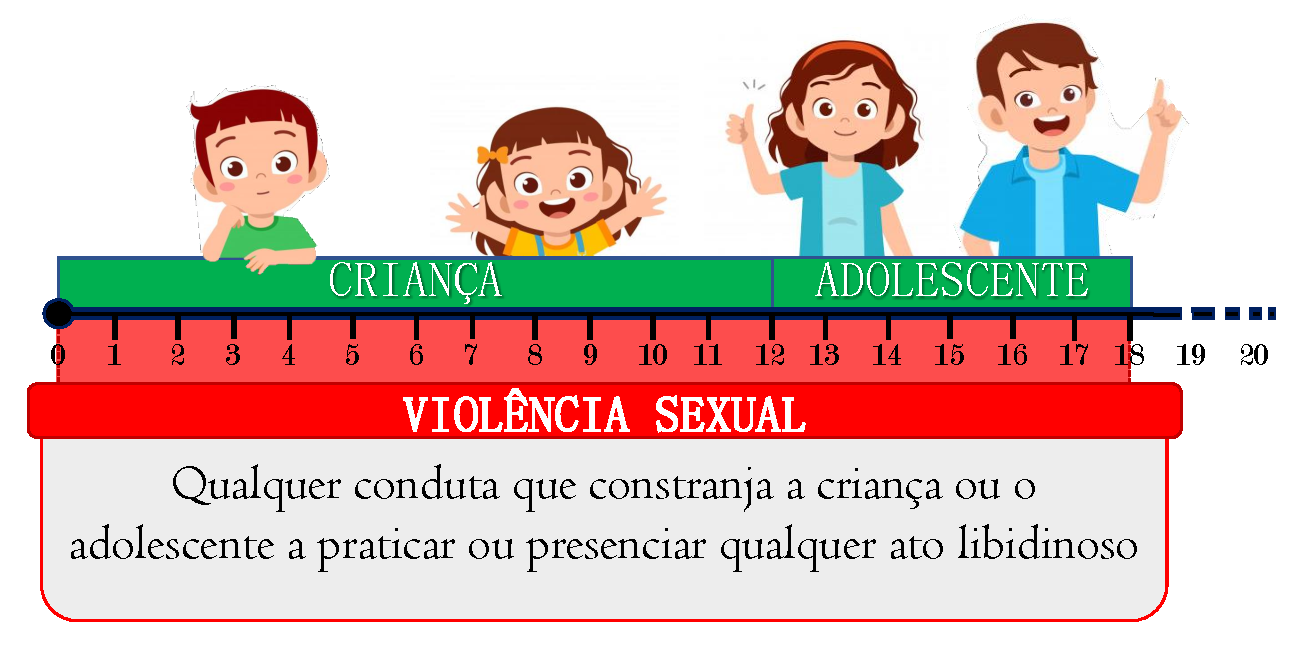
\includegraphics[width=\textwidth]{./Visuais/DefinicaoViolencia.pdf}
	\fonte{Elaborada pelo autor (2020).}
\end{figure}

A \autoref{fig:DefinicaoViolencia} define os termos: criança, adolescente e violência sexual. Os termos apresentados são retratados com base nas definições jurídicas brasileiras. No Brasil, de acordo com o \ac{ECA}, compreende-se como \textbf{criança} todo indivíduo até 12 (doze) anos de idade incompletos e como \textbf{adolescente} todo o indivíduo entre 12 (doze) e 18 (dezoito) anos de idade \cite{Lei:8069:1990}. Qualquer conduta libidinosa forçada contra um menor de 18 (dezoito) anos é caracterizada como violência sexual. A legislação brasileira classifica a violência sexual contra as crianças e adolescentes em três categorias: abuso sexual, exploração sexual comercial e tráfico de pessoas \cite{Lei:13431:2017}.

A legislação brasileira considera como \textbf{exploração sexual comercial}, todas as condutas sexuais com menores de idade envolvendo remuneração ou compensação. O conceito de \textbf{tráfico de pessoas} se firma sobre essa definição, englobando todas as atividades coercivas cujo a finalidade seja a exploração sexual. Já o conceito de \textbf{abuso sexual} se assemelha com a definição de \textbf{violência sexual} na legislação brasileira, sendo considerado como abuso sexual de criança ou adolescente, quaisquer atos libidinosos praticados de maneira forçada com um destes grupos, ou ambos. Entende-se como ato libidinoso, toda ação de satisfação da libido do agente agressor ou de outrem \cite{Lei:13431:2017}. Tais atos se dividem em duas categorias, as atividades com contato físico e as atividades sem contato físico. É listado a seguir, um compilado dos principais tipos de abuso sexual encontrados na literatura: 

%\raggedright
\begin{parcolumns}[sloppy, distance=3em, colwidths={2=0.5\textwidth}]{2}
	\colchunk{\flushright \underline{Abuso sexual \textbf{sem} ($\times$) contato físico}}
	\colchunk{\flushright \underline{Abuso sexual \textbf{com} (\checkmark) contato físico}}
	\colplacechunks

	\colchunk{\begin{itemize}[leftmargin=0.5cm]\item[$\times$] \justify \textbf{Abuso sexual verbal:} consiste em conversas abertas sobre atividades sexuais, destinadas a despertar o interesse da criança ou chocá-la.\end{itemize}}
	\colchunk{\begin{itemize}[leftmargin=1.8cm]\item[\checkmark] \justify \textbf{Estupro:} prática sexual forçada envolvendo penetração vaginal ou anal, ou quaisquer outras formas de abuso sexual com contato físico.\end{itemize}}

	\colplacechunks

	\colchunk{\begin{itemize}[leftmargin=0.5cm]\item[$\times$] \justify \textbf{Exibicionismo:} consiste em mostrar os órgãos genitais para crianças ou adolescentes.\end{itemize}}
	\colchunk{\begin{itemize}[leftmargin=1.8cm]\item[\checkmark] \justify \textbf{Sexo oral:} atividade sexual envolvendo contato entre a boca e os órgãos genitais (felação ou cunilíngua).\end{itemize}}

	\colplacechunks

	\colchunk{\begin{itemize}[leftmargin=0.5cm]\item[$\times$] \justify \textbf{Voyeurismo:} observar as genitálias da criança contra a vontade dela.\end{itemize}}
	\colchunk{\begin{itemize}[leftmargin=1.8cm]\item[\checkmark] \justify \textbf{Masturbação:} estimulação manual dos órgãos genitais da criança.\end{itemize}}

	\colplacechunks

	\colchunk{\begin{itemize}[leftmargin=0.5cm]\item[$\times$] \justify \textbf{Grooming:} consiste no aliciamento de crianças por meios eletrônicos.\end{itemize}}
	\colchunk{\begin{itemize}[leftmargin=1.8cm]\item[\checkmark] \justify \textbf{Aliciamento sexual:} suborno sexual mediante dinheiro ou poder.\end{itemize}}

	\colplacechunks

	\colchunk{\begin{itemize}[leftmargin=0.5cm]\item[$\times$] \justify \textbf{Sexting:} compartilhamento de conteúdo erótico por meios eletrônicos.\end{itemize}}
	\colchunk{\begin{itemize}[leftmargin=1.8cm]\item[\checkmark] \justify \textbf{Importunação sexual:} ato sexual sem a anuência dos envolvidos.\end{itemize}}
\end{parcolumns}

\newpage

A literatura revela uma quantidade expressiva de práticas sexuais abusivas \cite{brasil2002notificacao, habigzang2005abuso, sayao2006refazendo, santos2011guia, ibiapina2013influencias, lima2013violencia, lima2015violencia, barros2016participaccao, brasil2018violencia}. Salienta-se neste sentido, que outros tipos de abuso sexual não listados por este trabalho encontram-se devidamente documentados na literatura base. Existe inclusive uma compreensão mais ampla de abuso sexual com contato físico em alguns estudos, que inclui contatos forçados como beijos e toques em algumas zonas corporais erógenas \cite{sayao2006refazendo, santos2009guia}.

No Brasil, os atos praticados ou tentados de abuso sexual são punidos pela legislação brasileira. Eles podem ser legalmente tipificados em: rufianismo, corrupção de menor, assédio sexual, estupro de vulnerável, dentre outros \cite{Lei:12015:2009}. Destaca-se que diferentemente do crime de \textbf{estupro}, que exige constrangimento mediante violência ou grave ameaça, o \textbf{estupro de vulnerável} é crime mesmo com o consentimento da vítima, sendo considerado vulnerável, todo menor de 14 (catorze) anos ou pessoa incapacitada de oferecer qualquer tipo de resistência. 

A idade de 14 (catorze) anos estabelece a idade de consentimento mínima para a consumação de relações sexuais no Brasil. Salienta-se, no entanto que não há consenso entre os países acerca a idade de consentimento, podendo variar de região para região \cite{waites2005age}. Em alguns países o consentimento se configura no momento do matrimônio, independentemente da idade e anuência dos nubentes. 

Os atos consumados de abuso sexual são capazes de sequelar suas vítimas tanto fisicamente, quanto emocionalmente. Além disso, uma criança violentada pode chegar em sua fase adulta apresentando os mais variados transtornos e distúrbios \cite{mariscal2003programa, OMS2017responding}. Um achado das principais sequelas do abuso sexual, retratado pela bibliografia na área, é elencado a seguir:

%\raggedright
\begin{parcolumns}[sloppy, distance=3em, colwidths={2=0.35\textwidth}]{2}
	\colchunk{\flushleft \hspace{0.4cm} \underline{Sequelas \textbf{fisiológicas} ($\bullet$)}}
	\colchunk{\flushleft \underline{Sequelas \textbf{comportamentais} ($\circ$)}}
	\colplacechunks
	
	\colchunk{\begin{itemize}[leftmargin=0.5cm]\item[$\bullet$] \justify Gravidez\end{itemize}}
	\colchunk{\begin{itemize}[leftmargin=0.0cm]\item[$\circ$] \justify Depressão\end{itemize}}
	
	\colplacechunks
	
	\colchunk{\begin{itemize}[leftmargin=0.5cm]\item[$\bullet$] \justify Hemorragia\end{itemize}}
	\colchunk{\begin{itemize}[leftmargin=0.0cm]\item[$\circ$] \justify Retraimento\end{itemize}}

	\colplacechunks
	
	\colchunk{\begin{itemize}[leftmargin=0.5cm]\item[$\bullet$] \justify Hematomas\end{itemize}}
	\colchunk{\begin{itemize}[leftmargin=0.0cm]\item[$\circ$] \justify Ideação suicida\end{itemize}}

	\colplacechunks
	
	\colchunk{\begin{itemize}[leftmargin=0.5cm]\item[$\bullet$] \justify Lesões anais\end{itemize}}
	\colchunk{\begin{itemize}[leftmargin=0.0cm]\item[$\circ$] \justify Distúrbios do sono\end{itemize}}
	
	\colplacechunks
	
	\colchunk{\begin{itemize}[leftmargin=0.5cm]\item[$\bullet$] \justify Incontinência anal\end{itemize}}
	\colchunk{\begin{itemize}[leftmargin=0.0cm]\item[$\circ$] \justify Enurese e encoprese\end{itemize}}
	
	\colplacechunks
	
	\colchunk{\begin{itemize}[leftmargin=0.5cm]\item[$\bullet$] \justify Lesões geniturinárias\end{itemize}}
	\colchunk{\begin{itemize}[leftmargin=0.0cm]\item[$\circ$] \justify Transtorno alimentar\end{itemize}}
	
	\colplacechunks
	
	\colchunk{\begin{itemize}[leftmargin=0.5cm]\item[$\bullet$] Infecções sexualmente transmissíveis\end{itemize}}
	\colchunk{\begin{itemize}[leftmargin=0.0cm]\item[$\circ$] \justify Onanismo compulsivo\end{itemize}}
\end{parcolumns}

A bibliografia retrata uma quantidade significativa de traumas recorrentes de eventos sexuais abusivos \cite{OMS2003guidelines, mariscal2003programa, santos2011guia, pavao2013impasse, acuna2014abuso, deslandes2016atendimento}. Informa-se neste contexto, que demais sequelas não elencadas neste trabalho encontram-se devidamente documentadas na literatura da área. Há inclusive registros que relatam como consequência do abuso sexual na infância: agressividade, delinquência, autoflagelação, hipervigilância, hipovigilância, drogadição, estresse pós-traumático, transtorno do pânico e até mesmo a morte \cite{meurer2017direitos}. 

As sequelas do abuso sexual variam com base em certas condições, dentre elas: a idade da criança no início da violência; a duração e quantidade de ocorrências do abuso; o nível da violência; a diferença de idade entre os envolvidos e o vínculo entre criança e agressor \cite{florentino2015possiveis}. A maneira como essas condições ocorrem influenciam diretamente nos efeitos trágicos do abuso, isso pois, para as crianças menores, os sintomas tendem a se agravar mais devido a disparidade de tamanho entre os órgãos da criança e os órgãos do agressor. Além disso, a alta maleabilidade do encéfalo infantil permite que experiências negativas tenham maior probabilidade de causar danos graves e permanentes ao indivíduo \cite{pereira2011crescimento}. Registros informam inclusive que cerca de 90\% das pessoas com problemas psiquiátricos, sofreram alguma forma de maltrato na infância, sendo o abuso sexual, a forma de maltrato mais predominante relatada. Embora o abuso sexual seja largamente relatado em indivíduos com problemas psiquiátricos, é importante destacar que algumas crianças passam pelo abuso sem apresentar as sequelas descritas na literatura especializada \cite{aded2006abuso}. 

O abuso sexual de crianças traz consequências para toda civilização. A \ac{OMS} afirma inclusive que o abuso sexual é um grave problema de saúde pública a ser enfrentado por toda a sociedade \cite{OMS2017responding}. Estudos sobre sua incidência e prevalência mostram que esse fenômeno traz consequências que impactam significativamente a qualidade de vida das vítimas e de suas famílias, além de gerar altos custos econômicos para o país \cite{pinto2017avaliaccao}. Em resposta a esse fenômeno, incontáveis iniciativas surgiram ao redor do globo, voltadas à proteção dos direitos das crianças e dos adolescentes \cite{finkelhor2009prevention}.

No Brasil, o combate ao \ac{ASI} assume inúmeras formas, como: campanhas governamentais\footnote{A campanha \textbf{Não engula o choro} é uma iniciativa do estado do Paraná composta por animações e panfletos objetivados a sensibilizar a sociedade sobre o enfrentamento à violência e às violações de direitos das crianças.}, operações policiais\footnote{A \textbf{Operação Luz na Infância} é uma operação policial de âmbito internacional para à prevenção e enfrentamento de crimes cibernéticos relacionados ao abuso e exploração sexual de crianças e adolescentes.} e canais de denúncia\footnote{O \textbf{Disque 100} é um canal de comunicação para denúncias de violação de direitos humanos.}. Todavia, as estratégias do governo brasileiro não parecem surtir efeito no combate ao abuso sexual de crianças e adolescentes. Isso, pois as taxas anuais do abuso sexual mais que dobrando em um período inferior ao de uma década. A \autoref{fig:HistoricoViolencia} ilustra a aparente ineficiência das estratégias governamentais, com os registros da década de 2010 revelando um aumento quase que contínuo nos índices de abuso sexual de crianças e adolescentes.

\begin{figure}[!t]
	%\centering
	\caption{Panorama do abuso sexual infantil no Brasil.}\label{fig:HistoricoViolencia}
    \hspace{-4.8 cm}
    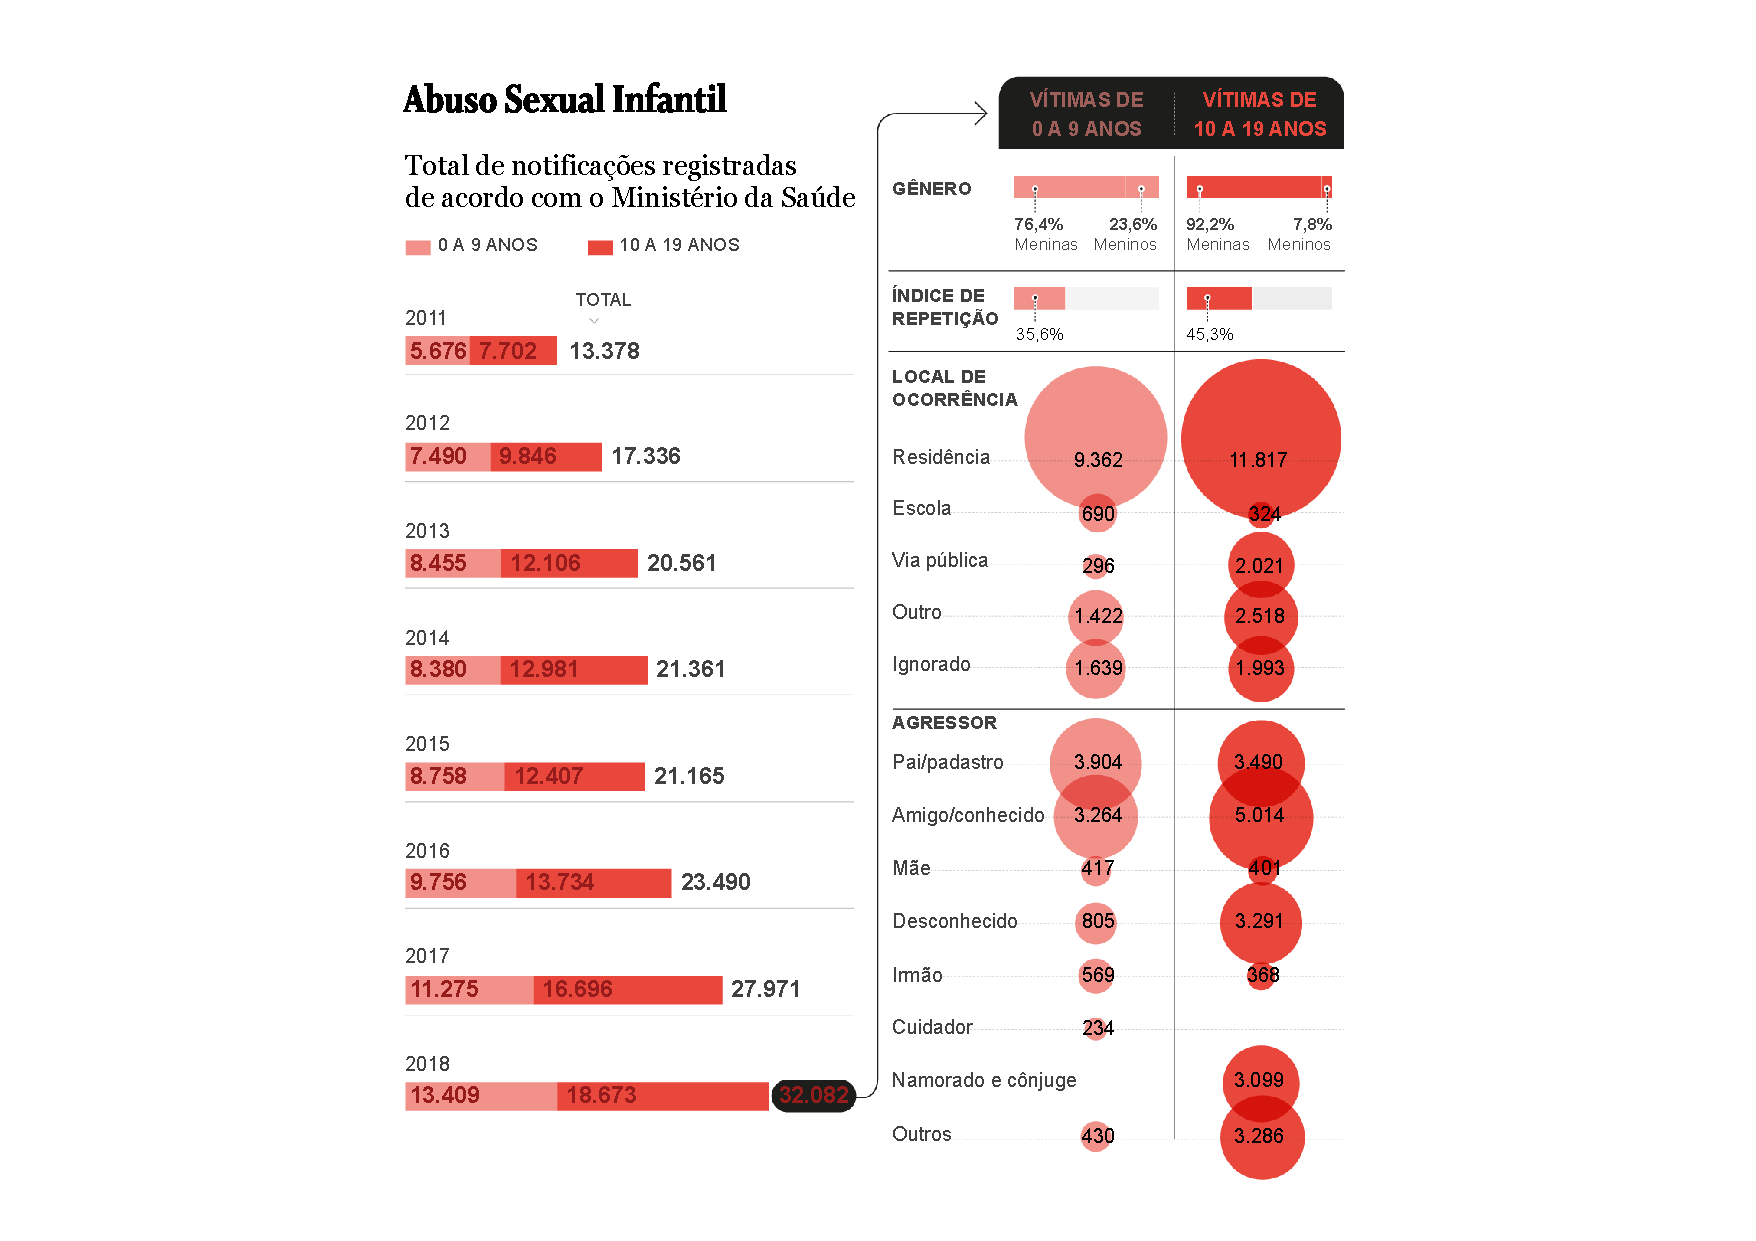
\includegraphics[width=1.6\linewidth]{./Visuais/HistoricoViolencia.pdf}
  	\vspace{-1.0cm}
	\fonte{Adaptado de \citeonline{globo2020tres}.}
\end{figure}

A \autoref{fig:HistoricoViolencia} apresenta a extensão do \ac{ASI} no Brasil. Os dados do DataSus\footnote{O DataSus é um departamento do Ministério da Saúde (MS) com a responsabilidade de coletar, processar e disseminar informações sobre a saúde nacional: \url{https://datasus.saude.gov.br/acesso-a-informacao/doencas-e-agravos-de-notificacao-de-2007-em-diante-sinan/}.} revelam um aumento expressivo na quantidade de notificações de abuso sexual de crianças, adolescentes e jovens adultos, entre os anos de 2011 e 2018. Os dados governamentais, além de apresentarem a totalidade das notificações distribuídas por ano, também filtra seus resultados por gênero, faixa etária, local de ocorrência, agressor, e outros tipos. 

Os dados governamentais demonstram um considerável aumento no número das notificações de violência sexual infantil no intervalo que abrange os anos de 2011 e 2018. Tal aumento pode indicar uma provável ineficiência das estratégias nacionais no combate ao \ac{ASI}. Contudo, cabe destacar que o ano de 2011 marca início de uma portaria\footnote{\label{note:nota0}Portaria Nº 1.171 de 19 de maio de 2011. Art. 2º Fica determinado que todos os estabelecimentos de saúde situados no território nacional, públicos e privados, integrantes ou não do Sistema Único de Saúde (SUS), devem informar ao Ministério da Saúde (MS), por intermédio dos gestores Municipais ou Estaduais, a ocorrência de todas as internações, independente de qualquer que seja a fonte de remuneração dos serviços prestados. Disponível em: \url{https://bvsms.saude.gov.br/bvs/saudelegis/gm/2011/prt1171_19_05_2011_rep.html}.} que obriga os agentes de saúde a notificar ao \ac{MS} todos os atendimentos. A portaria em si, tem como objetivo mitigar a questão da subnotificação dos dados, além de outras questões. Sendo assim, o aumento das notificações de violência sexual infantil após o ano de 2011 poderia ser um resultado da portaria, onde informações que estavam sendo subnotificadas passaram a serem notificadas. Contudo, pesquisas posteriores a portaria apontaram que somente 10\% dos casos de violência sexual são notificados às autoridades \cite{brasil2020abuso}. 

A subnotificação faz com que apenas uma parcela do problema seja revelada. O problema do \ac{ASI} manifesta-se então como um \textit{iceberg}, sendo a ponta do \textit{iceberg} a parte conhecida e notificada do problema e a parte submersa do \textit{iceberg} todos os casos não notificados. A subnotificação interfere diretamente na quantificação dos dados e na compreensão da dimensão do problema \cite{deslandes2016atendimento, hora2017violencia}. Dentre os principais motivos da subnotificação cita-se: o medo de represálias, o receio do estigma social, o descrédito dos agentes de saúde (antes da portaria\footref{note:nota0}) e a inscícia infantil \cite{fbsp2019anuario, pavao2013impasse}. %iceberg = geleira?

A inscícia das crianças acaba sendo um fator chave da subnotificação do problema. Em alguns casos a baixa vivência da criança faz com que o menor acabe por interpretar o abuso sexual sofrido com uma manifestação de carinho ou como uma prática normal \cite{aded2006abuso}. Em outros casos existe a inaptidão do menor em realizar o processo de denúncia, com a denúncia não sendo formalizada devido ao desconhecimento do processo legal por parte da criança \cite{OMS2002world}. Além disso, a incompreensão dos tramites legais pode levar a pensamentos incertos no que diz respeito ao sustento da casa, relacionado a seu provedor. As estratégias do governo brasileiro de combate ao \ac{ASI} falham nesse sentido, pois são praticamente incapazes de alcançar uma criança violentada sob estas condições, sendo uma das únicas formas de salvação da criança, a realização da denúncia por um terceiro. Além disso, tais estratégias, comumente se baseiam no princípio que o abuso já tenha ocorrido, enfatizando que a denúncia ainda se faz válida para episódios tentados (ou suspeitos) de abuso sexual.

O \ac{ASI} não é tratado com o rigor necessário pelo governo brasileiro. Grande parte das estratégias nacionais enfrentam o problema do abuso sexual de forma corretiva e não de maneira preventiva. A dificuldade das crianças em manifestar a violência sofrida acaba prejudicando as medidas tomadas pelas organizações nacionais. Sendo assim, uma das forma de contornar este empecilho vem por meio da conscientização de crianças, forma a qual já é aplicada em vários países \cite{plummer1999history, muller2014child}.

O Brasil aplica a conscientização de crianças no combate às drogas. A conscientização é realizada pelo \ac{PROERD}\footnote{O Programa Educacional de Resistência às Drogas e à Violência promove curso de quatro meses, ministrado por policiais militares voluntários, capacitados pedagogicamente, em parceria com pais, professores, estudantes e comunidades. Com ênfase na prevenção ao uso de drogas, as aulas mostram aos estudantes do quinto ano do ensino fundamental das redes pública e particular como se manter longe de más companhias, como evitar a violência, como resistir às pressões diretas ou indiretas e como acionar os pais ou responsáveis quando necessário. Mais informações sobre o programa podem ser encontradas em: \url{http://portal.mec.gov.br/ultimas-noticias/211-218175739/15910-programa-mostra-a-estudantes-como-ficar-longe-das-drogas}.}. Embora a temática da violência seja abordada, a violência sexual não é devidamente tratada pelo programa em questão. Para combater de maneira efetiva o problema do \ac{ASI} no Brasil é necessário a instauração de um programa educacional sólido de prevenção à violência sexual infantil que capacite e conscientize as crianças. 

Inúmeros estudos apontam como consequência benéfica dos programas de prevenção do \ac{ASI} a redução da incidência nos casos de abusos sexuais no médio e longo prazo \cite{maria2010papel}. Uma metanálise internacional informa inclusive que crianças capacitadas por programas do gênero possuem de seis a sete vezes mais chances de apresentarem repulsão a episódios de abuso (simulados) em comparação à crianças não capacitadas \cite{finkelhor2009prevention}. Outros 27 (vinte e sete) estudos revelam também que os programas são eficazes na construção do conhecimento das crianças acerca do abuso sexual e suas habilidades preventivas \cite{collin2013lessons}. 

Iniciativas preventivas de combate ao \ac{ASI} ajudam a evitar a ocorrência de episódios abusivos. Não faltam evidências que comprovam os resultados benéficos dos programas de prevenção e combate ao \ac{ASI} \cite{maria2010papel}. Diante deste fato, implementar um programa de educação nas escolas que prepare as crianças a coibir o abuso sexual é uma excelente maneira de prevenir abusos contra crianças e adolescentes \cite{santos2009guia}. Todavia, a temática do abuso sexual é extremamente sensível e delicada. A tarefa de ministrar tal conteúdo em salas de aula, pode acabar se tornando uma tarefa árdua e complicada. Como facilitador, surgem as estratégias pedagógicas baseadas em jogos. 

Estratégias baseadas em jogos didáticos vêm a agregar e facilitar o aprendizado infantil, principalmente em temas difíceis de abordar, devido aos tabus e aos preconceitos que os permeiam \cite{miranda2018abordagem}. As abordagens baseadas em jogos trazem diversão para temáticas sensíveis e pesadas, deixando os conteúdos apresentados e ensinados menos desagradáveis e incômodos. 

Jogos didáticos fornecem um meio poderoso de aprendizagem proporcionando uma maior motivação, confiança, engajamento e envolvimento dos alunos na aprendizagem, além de garantir um aprimoramento de suas habilidades \cite{colleen2016advancing}. Jogos associados a educação apresentam uma série de benefícios e vantagens. Entretanto, trazem algumas desvantagens como custos associados a produção, manutenção e treinamento. Como forma de contornar estes gastos, surgiram os jogos didáticos digitais.

\pagebreak

Os jogos didáticos digitais são ótimos facilitadores do processo pedagógico, pois herdam todas as vantagens associadas aos jogos físicos, sem herdar totalmente suas desvantagens. O principal empecilho que surge no lugar, diz respeito ao alcance dos jogos digitais. Em um cenário como o do Brasil, os jogos didáticos digitais enfrentam barreiras tecnológicas e econômicas. Um jogo didático digital, requer que o jogador possua um aparelho compatível com o jogo e conexão com a \textit{internet} (além de energia elétrica). A conexão com a \textit{internet} se faz necessária para o envio de informações sobre o desempenho do jogador no jogo a um banco de dados. Visando minimizar essas barreiras, soluções tecnológicas surgiram, como os jogos para navegadores. 

Os jogos para navegadores diminuem os requisitos necessários para a execução de um jogo. Entretanto, uma conexão via servidor ainda se faz indispensável neste tipo de aplicação. Felizmente, o Brasil tem ampliado cada vez mais o número de indivíduos conectados à \textit{internet}. Em 2019, a porcentagem de crianças e adolescentes conectados à rede alcançava os 89\% de toda essa população (entre nove e dezessete anos) \cite{nic2019pesquisa}. A expansão do número de usuários conectados à rede, viabiliza a instauração de um programa nacional preventivo de combate ao \ac{ASI} totalmente baseado na ideia de jogos para navegadores. Há inclusive, registro em vários países, de jogos do gênero sendo aplicados com sucesso na prevenção e no combate da violência sexual de crianças e adolescentes \cite{jones2008online, fingerle2018abschlussbericht}. 

Os jogos para navegadores voltados à prevenção e ao combate à violência sexual infantil, demonstram sucesso expressivo no ensino de habilidades preventivas. Os conceitos abordados por tais jogos assumem um importante papel no combate a violência sexual infantil. A oportunidade das crianças em praticar tais conceitos por intermédio de jogos fortalece ainda mais a luta contra os maus-tratos de meninas e meninos \cite{collin2013lessons}. A abordagem preventiva por meio de jogos digitais demonstra-se promissora no combate desse problema que assola tanto o Brasil, quanto o mundo. 

O enfretamento e a efetiva diminuição no número de casos de \ac{ASI} pode ser alcançado por intermédio de jogos educacionais para navegadores com temática preventiva a violência sexual infantil. Contudo, para isso, se faz necessário que tais jogos cumpram com certos requisitos, a fim de comprovar seus benefícios e justificar sua utilização por crianças de modo geral \cite{campos1996dez}. Sendo assim, jogos educacionais devem passar por um processo avaliativo para que sua eficácia pedagógica seja constatada, averiguando desta forma, se cada lição do jogo consegue cumprir com aquilo que foi planejado para ele \cite{montilva2002method, padron2007towards}. No caso de jogos com temática sensível, um processo avaliativo devidamente conduzido é capaz também de auxiliar na identificação de eventuais desconfortos que um jogo possa causar. Um jogo que seja rejeitado pelo processo avaliativo deve ter seu desenvolvimento retomado para corrigir eventuais falhas constatadas. Entretanto, um jogo de caráter preventivo a violência sexual infantil, aprovado pelo processo avaliativo, possui grande potencial para fortalecer os esforços na luta contra a violência sexual de crianças e adolescentes. 

%Objetivando combater a violência sexual de crianças, a atual pesquisa desenvolve um jogo digital para compor um programa preventivo de combate a violência sexual infantil. O jogo assenta seu desenvolvido em conceitos e estratégias encontradas nas bases da literatura pesquisa. Buscando averiguar a eficácia do programa, a atual pesquisa realiza experimentos com um amostra de crianças. Espera-se que a implementação de tal estratégia impacte, a curto prazo, nas habilidades e nos conhecimentos das crianças envolvidas no programa. A longo prazo, conjectura-se que haja uma diminuição das taxas de violência sexual infantil a nível nacional. 


%-------------------------------------------------------------------------------------------------------------------

\section{Objetivos}\label{sec:Objetivos}

O principal objetivo da presente pesquisa consiste em estabelecer uma estratégia eficaz no combate a violência sexual infantil. Nacionalmente, existem propostas de estratégias semelhantes as existentes no exterior, as quais apresentam grande sucesso \cite{steiler2012orbit, jones2020serious}. A atual pesquisa acredita que uma estratégia totalmente nacional devidamente adaptada a cultura e a realidade brasileira possui maiores chances de sucesso, em frente a uma estratégia estrangeira importada. Por tal razão, a presente pesquisa assenta suas ideias com base na estratégia educativa nacional proposta por \citeonline{diocesano2018infancia}.

\citeonline{diocesano2018infancia} propõe um jogo educacional para prevenção da violência sexual infantil, denominado de \textbf{Infância Segura}. O jogo em questão se destaca frente as outras propostas nacionais, pois possui uma quantidade superior de dinâmicas e uma maior variedade de temas tratados. Além disso, as temáticas abordadas pelo jogo proposto por \citeonline{diocesano2018infancia} obedecem à orientações internacionais de educação em sexualidade \cite{unesco2018international}. Sendo assim, essa pesquisa elege o jogo \textbf{Infância Segura} para ser desenvolvido e implementado em um programa educacional infantil para prevenção da violência sexual.

Como pesquisa científica, se busca a validação do programa educacional desenvolvido por meio de estudos, análises e experimentos. Uma pesquisa científica não diz respeito pura e simplesmente a construção de artefato, mas sim, aos achados e as descobertas envolvendo este artefato \cite{wazlawick2014metodologia}. Deste modo, o jogo desenvolvido configura-se como objetivo específico da presente pesquisa, já a análise experimental deste jogo configura-se como objetivo geral do atual trabalho acadêmico. Para atingir o objetivo geral, conjecturou-se o \hyperref[hipotese]{seguinte} teste de hipótese:

\label{hipotese}
\begin{itemize}
	%\item \textbf{Hipótese Nula (H$_{0}$):} O conhecimento de crianças, sobre a prevenção da violência sexual, é mantido após serem submetidas ao programa educacional desenvolvido nessa pesquisa, tendo como comparação seus desempenhos na etapa de pré e pós-teste. 

	%\item \textbf{Hipótese Alternativa (H$_{1}$):} O conhecimento de crianças, sobre a prevenção da violência sexual, é ampliado após serem submetidas ao programa educacional desenvolvido nessa pesquisa, tendo como comparação seus desempenhos na etapa de pré e pós-teste.
	\item \textbf{Hipótese Nula (H$_{0}$):} O conhecimento sobre a prevenção da violência sexual de crianças, submetidas ao programa educacional desenvolvido nessa pesquisa (grupo experimental), não apresenta diferença estatística siginificativas entre os conhecimentos sobre prevenção de crianças não submetidas ao programa educacional desenvolvido (grupo controle).
	
	\item \textbf{Hipótese Alternativa (H$_{1}$):} O conhecimento sobre a prevenção da violência sexual de crianças, submetidas ao programa educacional desenvolvido nessa pesquisa (grupo experimental), é estatisticamente superior aos conhecimentos sobre prevenção de crianças não submetidas ao programa educacional desenvolvido (grupo controle). 
\end{itemize}


%\legend{\large\label{hipotese}\Large{\textbf{Hipótese de pesquisa}}}
%\begin{framed}
%	\noindent
%	{\fontfamily{cmr}\selectfont O programa educacional para a prevenção da violência sexual infantil desenvolvido nessa pesquisa gera, aos participantes do programa, uma resposta cognitiva sobre os conceitos abordados.}
%\end{framed}


As \hyperref[hipotese]{hipóteses apresentadas} visam validar ou invalidar o programa educacional desenvolvimento por esse trabalho como uma proposta de combate a violência sexual infantil. A avaliação de tal programa define o objetivo geral (objetivo primário) da atual pesquisa acadêmica. Já o seu desenvolvimento configura o objetivo específico (objetivo secundário) do atual trabalho. O processo de avaliação do programa educacional é descrito em maiores detalhes na \autoref{sec:Avaliativos}. Enquanto que o jogo que compõe o programa é descrito no \autoref{ch:Desenvolvimento}. Os resultados desta pesquisa, relacioandos as \hyperref[hipotese]{hipóteses} apresentadas são descritos no \autoref{ch:Avaliacao}.

%-------------------------------------------------------------------------------------------------------------------

\section{Delimitação}\label{sec:Escopo}

A atual pesquisa fundamenta seus alicerces no desenvolvimento e na validação de um programa educacional para prevenção da violência sexual infantil. O programa desenvolvido pelo corrente trabalho tem o intuito de ensinar à prevenção da violência sexual infantil para crianças entre 5 (cinco) e 8 (oito) anos de idade. A faixa etária estabelecida do programa segue as orientações internacionais da \ac{UNESCO}\footnote{O documento da UNESCO separa os conceitos pedagógicos em quatro faixas etárias distintas (5 a 8 anos; 9 a 12 anos; 12 a 15 anos e 15 a 18+ anos). A \ac{UNESCO} recomenda que para maximizar a aprendizagem, é necessário trabalhar tópicos múltiplos relativos à sexualidade de maneira apropriada para a idade no decorrer de vários anos, utilizando uma abordagem de currículo em espiral. O documento pode ser acessado por meio do seguinte endereço eletrônico: \url{https://unesdoc.unesco.org/ark:/48223/pf0000369308}.}. No mais, a faixa etária estabelecida por esse trabalho foca em um dos grupos etários mais violentados de acordo com as pesquisas (\autoref{fig:violeciaIdade}). Além disso, é nessa faixa etária que programas de prevenção são mais eficazes \cite{davis2000child}.

\begin{figure}[htb]
	%\centering
	\caption{Taxa de vítimas de estupro, por faixa etária, Brasil (2020).}\label{fig:violeciaIdade}
    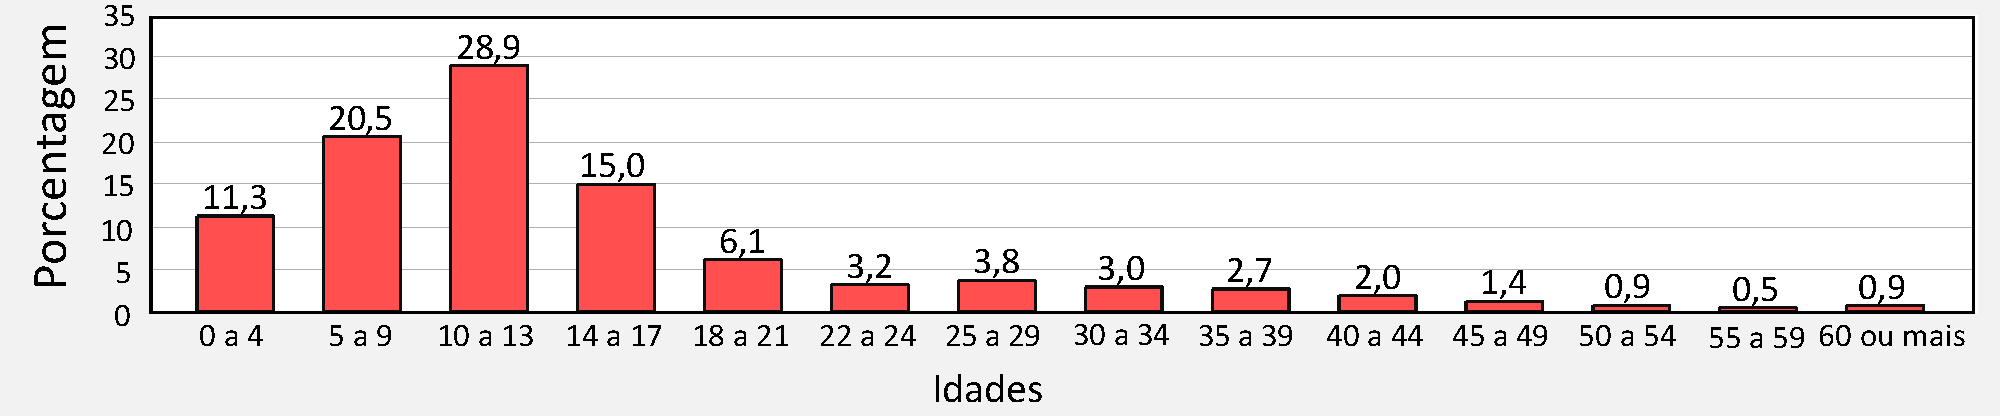
\includegraphics[width=\linewidth]{./Visuais/Idades1.pdf}
	\fonte{\citeonline{fbsp2021anuario}.}
	\vspace{-0.5cm}
\end{figure}


%É de notório saber que um programa sólido de educação sexual deve acompanhar a criança e o adolescente até sua fase adulta, contudo o atual trabalho abrange apenas a faixa etária mais tênue definida pela \ac{UNESCO}. A seleção da faixa etária mais tênue se deve pelo fato desta demarcar o início e a primeira etapa para os programas de educação sexual. Além disso, os prazos estabelecidos impedem que as demais etapas possam ser abordadas por essa pesquisa com a devida cautela e cuidado. Por tal razão, cabe a trabalhos futuros o desenvolvimento das demais etapas.

O programa educacional de prevenção a violência sexual infantil desenvolvido por essa pesquisa define sua estrutura pedagógica na forma de um jogo. Abordagens pedagógicas voltadas a prevenção da violência sexual infantil por meio de jogos já possuem resultados promissores em vários países \cite{muller2014child, fingerle2018abschlussbericht}. Além disso, tal abordagem ainda proporciona um sistema competente de acesso a informações positivas, confiáveis e livre de julgamentos sobre sexualidade e relacionamentos \cite{unesco2018international}. Desta forma, a abordagem por intermédio de jogos é eleita pela presente pesquisa para contemplar um programa educacional de prevenção a violência sexual infantil. 

O programa desenvolvido por essa pesquisa assenta seus conceitos pedagógicos e técnicos em documentos da literatura científica na área. Salienta-se que não se mensurou-se a efetiva contribuição de cada aspecto no processo de aprendizagem ou no processo técnico de desenvolvimento/validação. Os materiais usados para a elaboração, implementação e avaliação do programa desenvolvido não são julgados pela corrente pesquisa, sendo nesse sentido, o único papel do atual trabalho o de cumprir com as normas e diretrizes dos materiais base utilizados. 

%Em virtude da sensibilidade da temática tratada e do público-alvo vulnerável do corrente trabalho, informa-se da necessidade desta pesquisa em passar pelo Comitê de Ética. Após a aprovação da banca, os devidos tramites legais serão tomados para submeter essa pesquisa aos protocolos éticos cabíveis. 

Em virtude da sensibilidade da temática tratada e do público alvo vulnerável do corrente trabalho, informa-se que os procedimentos técnicos da presente pesquisa, envolvendo seres humanos (descritos na \autoref{sec:Avaliativos}), foram validados pelo Comitê de Ética em junho de 2021, sob o \ac{CAAE} nº 43602921.2.0000.0118. %https://www.udesc.br/arquivos/cct/id_cpmenu/1024/dissertacao_final_15167050734725_1024.pdf
% e seguiu as recomendações éticas vigentes, sobretudo guiadas pela Resolução 466/2012.

%-------------------------------------------------------------------------------------------------------------------
\newpage
\section{Metodologia da Pesquisa}\label{sec:Metodologia}

Para a construção dos conhecimentos desta pesquisa, se faz necessário definir um método a ser seguido. A seção de metodologia da pesquisa surge para trazer maior transparência aos processos e procedimentos que hão de culminar na conclusão de uma determinada pesquisa. Entender e classificar o tipo de pesquisa feita é fundamental para sustentar o planejamento e às decisões tomadas.

O presente trabalho classifica a corrente pesquisa com base nas classificações mais frequentes observadas em pesquisas atuais na área da ciência da computação. Deste modo a subseção \ref{sub:Natureza} menciona a natureza da atual pesquisa, a subseção \ref{sub:Recorte} delineia o tempo desta pesquisa, a subseção \ref{sub:Literatura} apresenta o método de revisão da literatura utilizado pela corrente pesquisa, a subseção \ref{sub:Abordagem} dá sua abordagem, a subseção \ref{sub:Metodo} detalha o método científico utilizado, a subseção \ref{sub:Procedimentos} explica seus procedimentos, a subseção \ref{sub:Finalidade} conta sua finalidade, a subseção \ref{sub:Maturidade} define o grau de maturidade e por fim, a subseção \ref{sub:Considerar} dá as considerações finais da atual seção. 


\subsection{Natureza}\label{sub:Natureza}

A natureza de um projeto de pesquisa vislumbra sobre o seu impacto na sociedade. Há, portanto, duas classificações: pesquisas básicas e pesquisas aplicadas. Pesquisas de natureza básica buscam o enriquecimento teórico do corpo científico. Já as pesquisas de natureza aplicada buscam por soluções para determinados problemas pragmáticos \cite{zanella2006metodologia}.

O corrente trabalho acadêmico almeja solucionar o problema da violência sexual infantil no Brasil. A solução pensada assume a forma de um programa educacional infantil focado na ensino-aprendizagem por meio da dinâmica de jogos. Espera-se que o programa capacite seus participantes de modo a coibirem e relatarem episódios de abuso culminando assim, na redução dos crimes. Definido o problema pragmático a ser tratado, afirma-se que a corrente pesquisa é de natureza aplicada.

\subsection{Recorte}\label{sub:Recorte}

O recorte de um estudo define a duração da pesquisa, podendo ser transversal ou longitudinal. Pesquisas transversais demarcam os estudos realizados em pontos específicos no tempo. Pesquisas longitudinais englobam um intervalo de tempo maior, analisando o durante, o antes e o depois da pesquisa \cite{hochman2005desenhos}. 

O corrente estudo opera em uma janela curta de tempo. As informações analisadas dizem respeito pura e simplesmente a dados colhidos durante o andamento do estudo, por tal razão a atual pesquisa remete a um recorte transversal no tempo. 

\subsection{Revisão da Literatura}\label{sub:Literatura}

A revisão da literatura diz respeito a pressupostos teóricos que dão fundamentação à pesquisa e as contribuições proporcionadas por investigações anteriores \cite{carlos2002elaborar}. Existem duas classificações nesse sentido: as tradicionais e as sistemáticas. As revisões tradicionais não utilizam critérios explícitos para a seleção das obras que hão de fundamentar a pesquisa. Já as revisões sistemáticas são as pesquisas que se utilizam de um processo rigoroso para a seleção de obras para sua fundamentação \cite{ferenhof2016desmistificando}.

O atual estudo conduz uma revisão da literatura tradicional, isenta de quaisquer critérios mais severos para a seleção de artigos. No entanto, o presente trabalho priorizou utilizar os seguintes \acfp{MBA}: ACM DL, IEEExplore, Science Direct e Web of Science. A escolha por esses \acp{MBA} deu-se por abrigarem publicações de qualidade reconhecida pela \ac{CAPES}. Também foram pesquisados periódicos, livros, revistas científicas e \textit{sites} de referência na área; além de consultadas as citações referenciadas durante toda a dissertação. Sendo assim, enfatiza-se que a presente pesquisa baseia sua revisão literária em obras científicas e revisadas por pares principalmente; mas também, em documentos e demais materiais sem tratamento prévio retornados durante a etapa de revisão da literatura. 

\subsection{Abordagem}\label{sub:Abordagem}

A abordagem metodológica de uma pesquisa informa a respeito da natureza de suas variáveis. Logo existem as pesquisas de abordagem quantitativa e as de abordagem qualitativa. Pesquisas quantitativas trabalham sumariamente com variáveis numéricas e objetivas. Já as pesquisas qualitativas trabalham majoritariamente com elementos subjetivos e abstratos \cite{carlos2002elaborar}. As pesquisas que contemplam ambos os tipos são categorizadas como pesquisas quanti-qualitativas ou pesquisas mistas. 

A atual pesquisa mensura o desempenho, a aprendizagem e o engajamento dos participantes envolvidos no processo de validação de um programa educacional. O desempenho (quantitativo) é colhido de maneira virtual por meio de arquivos gerados durante os experimentos realizados com o jogo desenvolvido; neste quesito informações como os acertos, erros e os tempos de resposta para os exercícios do jogo são colhidos. A aprendizagem (quantitativo) é mensurada através de um conjunto de questões focadas em medir o nível de conhecimento adquirido pelos participantes do programa. O engajamento (qualitativo) é alcançado por meio de entrevistas e depoimentos em um grupo focal com o intuito de identificar os níveis de agradabilidade do programa ao seu público-alvo. Definidas as variáveis mensuradas, afirma-se que o atual trabalho possui uma abordagem quanti-qualitativa. 

\subsection{Método}\label{sub:Metodo}

Na área da metodologia, o método define a forma de raciocínio lógico que guiará a pesquisa científica. Quatro formas de raciocínio se destacam: indutivo, dedutivo, hipotético-dedutivo e dialético. O método indutivo induz os achados específicos de uma pesquisa para um contexto geral. O método dedutivo deduz os conhecimentos gerais para contextos específicos. O método hipotético-dedutivo diz respeito as pesquisas baseadas em princípios de falseabilidade. O método dialético descreve os fenômenos de uma pesquisa \cite{marconi2003lakatos}.  

A atual pesquisa submete um programa educacional a um conjunto reduzido de participantes. Os resultados do conjunto são extrapolados para toda a população de maneira a validar ou invalidar a eficácia do programa. Logo, o presente estudo segue a corrente indutiva. 

\subsection{Procedimentos Técnicos}\label{sub:Procedimentos}

A metodologia divide os procedimentos técnicos em dois grupos distintos de coleta de dados. Há os grupos responsáveis pela coleta direta de informações e os responsáveis pela coleta indireta de informações. A coleta indireta de informações tende a ser realizada por pesquisas documentais ou bibliográficas. Já a coleta direta de informações corresponde normalmente a pesquisas experimentais ou etnográficas \cite{cordova2009pesquisa}. 

A atual pesquisa realiza a validação de um programa educacional com o auxílio de dois grupos de participantes, um grupo experimental e um grupo controle. Tal abordagem é associada a pesquisas experimentais. Todavia, salienta-se que os grupos selecionados pelo presente estudo não obedecem a uma distribuição aleatória (um dos fatores principais para a elaboração de pesquisas experimentais sólidas). %O processo avaliativo da presente pesquisa é composto unicamente por crianças da rede pública de ensino. A seleção exclusiva de participantes da rede pública de ensino resulta em um possível viés da pesquisa. 
%Por tal razão a atual pesquisa se enquadra em uma classe de pesquisas experimentais conhecidas como pesquisas quase-experimentais \apud{campbell1979delineamentos}{carlos2002elaborar}.
Pelo fato dos grupos selecionados serem compostos por indivíduos da mesma região e nível educacional (rede pública), a amostra utilizada não pode ser classificada como totalmente aleatória, sendo assim, a atual pesquisa se enquadra na classe das pesquisas quase-experimentais \apud{campbell1979delineamentos}{carlos2002elaborar}.

%POR NÃO TER MUITAS DIFERENÇAS ETNICAS OU SOCIO-ECONOMICAS A AMOSTRA NÃO É ALEATORIO, POR ISSO ESSA É UMA PESQUISA QUASE-EXPERIMENTAL. 

\subsection{Finalidade}\label{sub:Finalidade}

A  finalidade de uma pesquisa define a relação entre a pesquisa e um problema. Três relações se destacam: exploratória, descritiva e explicativa. As exploratórias buscam compreender e explorar melhor determinado problema. As descritivas almejam descrever o problema e identificar relações entre variáveis associadas ao problema. As explicativas procuram explicar e determinar os fatores que contribuem para a ocorrência do problema \cite{trivinos2009introduccao}. 

A atual pesquisa relaciona as variáveis de aprendizagem entre o grupo experimental e o grupo controle, se utilizando do Teste T (com 95\% de confiança). Como adicional, o presente estudo também relaciona as variáveis de desempenho e aprendizagem a fim de encontrar relações entre o desempenho de determinados indivíduos em um jogo e o aprimoramento de suas habilidades intelectuais no que diz respeito aos assuntos ministrados pelo jogo. Dada a relação das variáveis mensuradas, afirma-se que a corrente pesquisa é de finalidade descritiva.

\subsection{Nível de Maturidade}\label{sub:Maturidade}

A maturidade de uma pesquisa se divide em níveis de acordo com a observabilidade dos resultados em relação aos trabalhos existentes. O primeiro nível não apresenta nenhum comparativo, sendo a pura descrição do objeto estudado. O segundo nível realiza um comparativo empírico entre o objeto de estudo e demais existentes. O terceiro nível se utiliza de métricas novas para conduzir tal comparativo. O quarto nível se utiliza de métricas consolidadas. O quinto e último nível consiste na apresentação de uma teoria consistente sobre o objeto estudado \cite{wazlawick2014metodologia}.%. com as observações de forma coerente.

O presente trabalho acadêmico desenvolve um jogo para compor um programa educacional para prevenção da violência sexual infantil. O jogo desenvolvido é confrontado de maneira empírica com os demais jogos já existentes nesse cenário. Uma tabela comparativa é construída para proporcionar ao leitor maior clareza entre o artefato desenvolvido nessa pesquisa e demais já existentes. Desta forma, essa pesquisa alcança o segundo grau de maturidade. 


\subsection{Considerações}\label{sub:Considerar}

As classificações em metodologia permitem sustentar o planejamento e às decisões tomadas pelo corrente trabalho acadêmico. Os métodos e processos presentes no campo da metodologia auxiliam, não apenas na condução da pesquisa pelo pesquisador autor, mas também na análise e na revisão da pesquisa por demais pesquisadores da área.

O processo de classificação da corrente pesquisa, buscou fundamentação nos trabalhos citados nas respectivas subseções. Todavia, enfatiza-se que o processo de classificação, embora fundamentado, não está livre de falhas. Por tal razão, as classificações feitas, não devem ser vistas como absolutas, mas sim, como as classificações consideradas mais apropriadas identificadas pelo autor desta dissertação. Salienta-se que a presente seção buscou, apenas, classificar a presente pesquisa. Todos os procedimentos conduzidos para a realização da pesquisa e dos experimentos são descritos mais detalhadamente nas demais seções e capítulos desta dissertação.

%-------------------------------------------------------------------------------------------------------------------

\section{Estrutura do Trabalho}\label{ch:Estrutura}

A presente dissertação organiza sua redação em sete capítulos. O \autoref{ch:Introducao} dá uma breve descrição sobre a problemática a ser abordada, os objetivos da pesquisa e sua metodologia. O \autoref{ch:Fundamentacao} fundamenta algumas ideias essenciais para a compreensão e andamento da pesquisa, abordando desde a definição de Jogo Sério, metodologias para o desenvolvimento de jogos e modelos para a avaliação de programas voltados para a prevenção da violência sexual infantil. O \autoref{ch:Relacionados} apresenta algumas estratégias voltadas para o combate da violência sexual de crianças. O \autoref{ssec:TR} apresenta os trabalhos relacionados com a atual pesquisa. O \autoref{ch:Desenvolvimento} ilustra as questões de desenvolvimento do jogo elaborado, desde aspectos técnicos até aspectos pedagógicos. O \autoref{ch:Avaliacao} explica o processo de validação do jogo. Por fim, o \autoref{ch:Conclusao} finaliza a atual pesquisa com suas conclusões.

%-------------------------------------------------------------------------------------------------------------------





